% Options for packages loaded elsewhere
\PassOptionsToPackage{unicode}{hyperref}
\PassOptionsToPackage{hyphens}{url}
%
\documentclass[
]{article}
\usepackage{amsmath,amssymb}
\usepackage{iftex}
\ifPDFTeX
  \usepackage[T1]{fontenc}
  \usepackage[utf8]{inputenc}
  \usepackage{textcomp} % provide euro and other symbols
\else % if luatex or xetex
  \usepackage{unicode-math} % this also loads fontspec
  \defaultfontfeatures{Scale=MatchLowercase}
  \defaultfontfeatures[\rmfamily]{Ligatures=TeX,Scale=1}
\fi
\usepackage{lmodern}
\ifPDFTeX\else
  % xetex/luatex font selection
\fi
% Use upquote if available, for straight quotes in verbatim environments
\IfFileExists{upquote.sty}{\usepackage{upquote}}{}
\IfFileExists{microtype.sty}{% use microtype if available
  \usepackage[]{microtype}
  \UseMicrotypeSet[protrusion]{basicmath} % disable protrusion for tt fonts
}{}
\makeatletter
\@ifundefined{KOMAClassName}{% if non-KOMA class
  \IfFileExists{parskip.sty}{%
    \usepackage{parskip}
  }{% else
    \setlength{\parindent}{0pt}
    \setlength{\parskip}{6pt plus 2pt minus 1pt}}
}{% if KOMA class
  \KOMAoptions{parskip=half}}
\makeatother
\usepackage{xcolor}
\usepackage[margin=1in]{geometry}
\usepackage{color}
\usepackage{fancyvrb}
\newcommand{\VerbBar}{|}
\newcommand{\VERB}{\Verb[commandchars=\\\{\}]}
\DefineVerbatimEnvironment{Highlighting}{Verbatim}{commandchars=\\\{\}}
% Add ',fontsize=\small' for more characters per line
\usepackage{framed}
\definecolor{shadecolor}{RGB}{248,248,248}
\newenvironment{Shaded}{\begin{snugshade}}{\end{snugshade}}
\newcommand{\AlertTok}[1]{\textcolor[rgb]{0.94,0.16,0.16}{#1}}
\newcommand{\AnnotationTok}[1]{\textcolor[rgb]{0.56,0.35,0.01}{\textbf{\textit{#1}}}}
\newcommand{\AttributeTok}[1]{\textcolor[rgb]{0.13,0.29,0.53}{#1}}
\newcommand{\BaseNTok}[1]{\textcolor[rgb]{0.00,0.00,0.81}{#1}}
\newcommand{\BuiltInTok}[1]{#1}
\newcommand{\CharTok}[1]{\textcolor[rgb]{0.31,0.60,0.02}{#1}}
\newcommand{\CommentTok}[1]{\textcolor[rgb]{0.56,0.35,0.01}{\textit{#1}}}
\newcommand{\CommentVarTok}[1]{\textcolor[rgb]{0.56,0.35,0.01}{\textbf{\textit{#1}}}}
\newcommand{\ConstantTok}[1]{\textcolor[rgb]{0.56,0.35,0.01}{#1}}
\newcommand{\ControlFlowTok}[1]{\textcolor[rgb]{0.13,0.29,0.53}{\textbf{#1}}}
\newcommand{\DataTypeTok}[1]{\textcolor[rgb]{0.13,0.29,0.53}{#1}}
\newcommand{\DecValTok}[1]{\textcolor[rgb]{0.00,0.00,0.81}{#1}}
\newcommand{\DocumentationTok}[1]{\textcolor[rgb]{0.56,0.35,0.01}{\textbf{\textit{#1}}}}
\newcommand{\ErrorTok}[1]{\textcolor[rgb]{0.64,0.00,0.00}{\textbf{#1}}}
\newcommand{\ExtensionTok}[1]{#1}
\newcommand{\FloatTok}[1]{\textcolor[rgb]{0.00,0.00,0.81}{#1}}
\newcommand{\FunctionTok}[1]{\textcolor[rgb]{0.13,0.29,0.53}{\textbf{#1}}}
\newcommand{\ImportTok}[1]{#1}
\newcommand{\InformationTok}[1]{\textcolor[rgb]{0.56,0.35,0.01}{\textbf{\textit{#1}}}}
\newcommand{\KeywordTok}[1]{\textcolor[rgb]{0.13,0.29,0.53}{\textbf{#1}}}
\newcommand{\NormalTok}[1]{#1}
\newcommand{\OperatorTok}[1]{\textcolor[rgb]{0.81,0.36,0.00}{\textbf{#1}}}
\newcommand{\OtherTok}[1]{\textcolor[rgb]{0.56,0.35,0.01}{#1}}
\newcommand{\PreprocessorTok}[1]{\textcolor[rgb]{0.56,0.35,0.01}{\textit{#1}}}
\newcommand{\RegionMarkerTok}[1]{#1}
\newcommand{\SpecialCharTok}[1]{\textcolor[rgb]{0.81,0.36,0.00}{\textbf{#1}}}
\newcommand{\SpecialStringTok}[1]{\textcolor[rgb]{0.31,0.60,0.02}{#1}}
\newcommand{\StringTok}[1]{\textcolor[rgb]{0.31,0.60,0.02}{#1}}
\newcommand{\VariableTok}[1]{\textcolor[rgb]{0.00,0.00,0.00}{#1}}
\newcommand{\VerbatimStringTok}[1]{\textcolor[rgb]{0.31,0.60,0.02}{#1}}
\newcommand{\WarningTok}[1]{\textcolor[rgb]{0.56,0.35,0.01}{\textbf{\textit{#1}}}}
\usepackage{longtable,booktabs,array}
\usepackage{calc} % for calculating minipage widths
% Correct order of tables after \paragraph or \subparagraph
\usepackage{etoolbox}
\makeatletter
\patchcmd\longtable{\par}{\if@noskipsec\mbox{}\fi\par}{}{}
\makeatother
% Allow footnotes in longtable head/foot
\IfFileExists{footnotehyper.sty}{\usepackage{footnotehyper}}{\usepackage{footnote}}
\makesavenoteenv{longtable}
\usepackage{graphicx}
\makeatletter
\def\maxwidth{\ifdim\Gin@nat@width>\linewidth\linewidth\else\Gin@nat@width\fi}
\def\maxheight{\ifdim\Gin@nat@height>\textheight\textheight\else\Gin@nat@height\fi}
\makeatother
% Scale images if necessary, so that they will not overflow the page
% margins by default, and it is still possible to overwrite the defaults
% using explicit options in \includegraphics[width, height, ...]{}
\setkeys{Gin}{width=\maxwidth,height=\maxheight,keepaspectratio}
% Set default figure placement to htbp
\makeatletter
\def\fps@figure{htbp}
\makeatother
\ifLuaTeX
  \usepackage{luacolor}
  \usepackage[soul]{lua-ul}
\else
  \usepackage{soul}
\fi
\setlength{\emergencystretch}{3em} % prevent overfull lines
\providecommand{\tightlist}{%
  \setlength{\itemsep}{0pt}\setlength{\parskip}{0pt}}
\setcounter{secnumdepth}{-\maxdimen} % remove section numbering
\ifLuaTeX
  \usepackage{selnolig}  % disable illegal ligatures
\fi
\usepackage{bookmark}
\IfFileExists{xurl.sty}{\usepackage{xurl}}{} % add URL line breaks if available
\urlstyle{same}
\hypersetup{
  pdftitle={Markdown Commands},
  pdfauthor={Noah W.K. Mattheis},
  hidelinks,
  pdfcreator={LaTeX via pandoc}}

\title{Markdown Commands}
\author{Noah W.K. Mattheis}
\date{2025-01-21}

\begin{document}
\maketitle

Ok so I can just type as I normally would for any text, no marks needed.
Always seperate paragraphs with two carriage returns.

Here is our second paragraph.

Header size determined by number of ``\#'' with less being larger font

\section{First header (largest)}\label{first-header-largest}

\subsection{If done this way, will print all in one
line}\label{if-done-this-way-will-print-all-in-one-line}

Noah Mattheis Pharmacology MS Student University of Vermont

\subsection{Second Level (getting smaller in
size)}\label{second-level-getting-smaller-in-size}

\subsection{need two spaces between them for lines
between}\label{need-two-spaces-between-them-for-lines-between}

\subsubsection{Third level}\label{third-level}

\paragraph{Fourth level}\label{fourth-level}

Noah Mattheis

Pharmacology MS Student

University of Vermont

Use \emph{astericks} for \emph{italic} and \textbf{double astericks} for
\textbf{bold}

Use \textsuperscript{caret} `\^{}' for \textsuperscript{superscript} and
\textsubscript{tilda} `\textasciitilde{}' for \textsubscript{subscript}
and \st{2 tildas} '\textasciitilde\textasciitilde'for \st{strikethrough}

Use r in an in-line text:

The value of pi + 10 is 13.1415927.

\begin{quote}
Use a greater than sign for indented quoted material. Looks nice
Ceaser-chan!
\end{quote}

\subsection{For Lists}\label{for-lists}

\begin{itemize}
\tightlist
\item
  first item
\item
  second item

  \begin{itemize}
  \tightlist
  \item
    indented list item
  \item
    also indented item
  \end{itemize}
\end{itemize}

\subsection{For Links}\label{for-links}

links \href{website\%20address}{linking text} Lets try for my favorite
magic card art

Bearer of the Heavens
\href{https://gatherer.wizards.com/pages/card/details.aspx?name=Bearer\%20of\%20the\%20Heavens}{Card}

\subsection{For Tables}\label{for-tables}

\begin{longtable}[]{@{}ll@{}}
\toprule\noalign{}
First Header & Second Header \\
\midrule\noalign{}
\endhead
\bottomrule\noalign{}
\endlastfoot
Content Cell & Content Cell \\
Content Cell & Content Cell \\
\end{longtable}

\subsection{Fencing Options}\label{fencing-options}

Use a single back tick/ backwards quotation mark for
\texttt{in\ line\ fencing} of material.

Use triple back tips for fenced block of text

\begin{verbatim}
Everything here is a plain text
even with markdown *commands*
Stays until closed with 3 back tips

Blank lines properly spaced

Very nice, Ceaser-chan
\end{verbatim}

\subsection{Important type of fencing}\label{important-type-of-fencing}

\paragraph{using chunk of r code - everything between the marks will be
executed as r
code}\label{using-chunk-of-r-code---everything-between-the-marks-will-be-executed-as-r-code}

\paragraph{will show code and execution of said
code}\label{will-show-code-and-execution-of-said-code}

\paragraph{if eval=FALSE, will not show code output, easier for sharing
code}\label{if-evalfalse-will-not-show-code-output-easier-for-sharing-code}

\paragraph{if eval=TRUE AND echo=FALSE, we will see output but not the
code}\label{if-evaltrue-and-echofalse-we-will-see-output-but-not-the-code}

\begin{verbatim}
##  [1] 0.2610814 0.7690179 0.4726754 0.1032719 0.4986805 0.7555883 0.1676998 0.9190942
##  [9] 0.0333595 0.9718758
\end{verbatim}

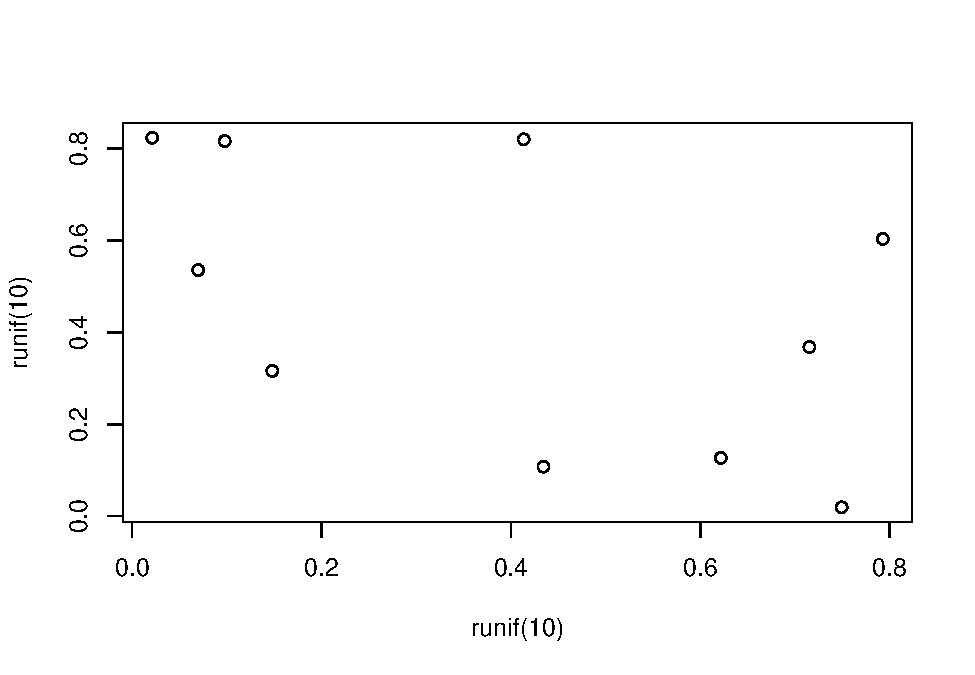
\includegraphics{FirstMarkdown_files/figure-latex/unnamed-chunk-1-1.pdf}

Having both be true

\begin{Shaded}
\begin{Highlighting}[]
\CommentTok{\# r code can be used here! }

\FunctionTok{print}\NormalTok{(}\FunctionTok{runif}\NormalTok{(}\DecValTok{10}\NormalTok{))}
\end{Highlighting}
\end{Shaded}

\begin{verbatim}
##  [1] 0.51849566 0.64577298 0.12100735 0.70719522 0.49258055 0.02658777 0.77927377 0.17460403
##  [9] 0.21122615 0.96134954
\end{verbatim}

\begin{Shaded}
\begin{Highlighting}[]
\FunctionTok{plot}\NormalTok{(}\FunctionTok{runif}\NormalTok{(}\DecValTok{10}\NormalTok{), }\FunctionTok{runif}\NormalTok{(}\DecValTok{10}\NormalTok{))}
\end{Highlighting}
\end{Shaded}

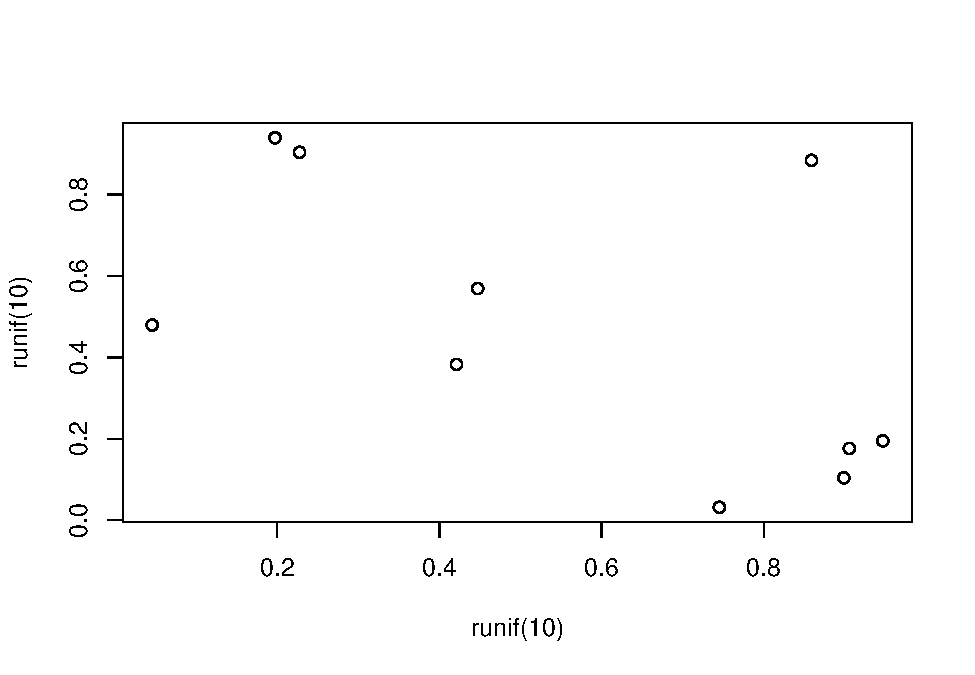
\includegraphics{FirstMarkdown_files/figure-latex/unnamed-chunk-2-1.pdf}

Having eval false here

\begin{Shaded}
\begin{Highlighting}[]
\CommentTok{\# r code can be used here! }

\FunctionTok{print}\NormalTok{(}\FunctionTok{runif}\NormalTok{(}\DecValTok{10}\NormalTok{))}
\FunctionTok{plot}\NormalTok{(}\FunctionTok{runif}\NormalTok{(}\DecValTok{10}\NormalTok{), }\FunctionTok{runif}\NormalTok{(}\DecValTok{10}\NormalTok{))}
\end{Highlighting}
\end{Shaded}

\subsection{Using LaTeX for Math, o ya
baby}\label{using-latex-for-math-o-ya-baby}

Use a single dollar sign at the beginning and end of equation
\(a = b + c\)

To insert a mathematical statement within plain text, no spaces OR use
double dollar signs, can be used with spaces, for center and separted
equation \[ a = b + c \] Subscripts, using '\_'

`H\_0'' important here \[H_0 = Z_{a + b}\] Superscripts, using a
caret'\^{}' \[S = cA^z\] Combining

\[S=cA^z_1 + z_{2 + x}\]

Fraction with variables

\[\alpha = \frac{\beta}{\delta + \gamma_x}\]

Summation signs

\[z = \sum_{i=1}^X{K}\] Just a backslash

\[\backslash\] backslash le gives us less than or equal to
\[\backslash \alpha \le b \backslash\]

Mixing text and equations, we need an m box, without it it will smush
text together and treat it all as one variable
\[P(\mbox{Occurence of Species A}) = Z\]

Back to chunkin'

\begin{Shaded}
\begin{Highlighting}[]
\CommentTok{\#Here is a new chunk of code, distant from the first one in our document.}

\NormalTok{z }\OtherTok{\textless{}{-}} \DecValTok{1}\SpecialCharTok{:}\DecValTok{10}
\FunctionTok{print}\NormalTok{(z)}
\end{Highlighting}
\end{Shaded}

\begin{verbatim}
##  [1]  1  2  3  4  5  6  7  8  9 10
\end{verbatim}

\begin{Shaded}
\begin{Highlighting}[]
\CommentTok{\#end of second chunk}
\end{Highlighting}
\end{Shaded}


\end{document}
